\chapter{Spin, phép đo và không gian trạng thái hai chiều}

\lectureoverview{Spin có tính định hướng, nhưng mỗi phép đo một trong các thành phần của nó chỉ cho kết quả \(+1\) hoặc \(-1\). Trước hết ta nêu rõ câu đố mang tính thao tác ấy, rồi xem vì sao logic tập hợp thông thường thất bại đối với các phép đo không tương thích. Một không gian vectơ phức hai chiều cung cấp ngôn ngữ thích hợp: xác suất xuất phát từ biên độ, các khả năng có thể phân biệt được thì trực giao, và các cơ sở lên--xuống, phải--trái, và vào--ra mã hóa ba hướng không gian mà không biến một vectơ trạng thái thành một mũi tên thông thường.}

\section{Từ qubit đến spin}

Hệ hai trạng thái được giới thiệu như một qubit từ đây sẽ được gọi là một \emph{spin}. Việc đổi tên đưa phương hướng không gian vào thảo luận, nhưng nó cũng tạo ra một nguy cơ gây nhầm lẫn với từ \emph{vectơ}. Cần phân biệt hai đối tượng khác nhau:

\begin{definition}
Một \emph{vectơ ba chiều} là một vectơ thực thông thường trong không gian ba chiều. Một \emph{vectơ} không kèm định ngữ sẽ có nghĩa là một phần tử của một không gian vectơ trừu tượng, chẳng hạn như không gian trạng thái phức dùng trong cơ học lượng tử.
\end{definition}

Một spin có thể được chuẩn bị theo một trục trong không gian thông thường. Tuy nhiên, trạng thái của nó sẽ được biểu diễn bằng một vectơ trừu tượng. Mối liên hệ giữa hai phát biểu ấy là một trong những điều ta phải khám phá; không thể giả định nó từ một hình vẽ.

\section{Vì sao không thể loại bỏ thiết bị}

Cơ học cổ điển khiến ta dễ hình dung một người quan sát lý tưởng có thể tìm hiểu một hệ trong khi gây nhiễu lên nó ít đến mức tùy ý. Chẳng hạn, giả sử ta muốn nhìn một vật vĩ mô. Ta chiếu sáng nó, thu ánh sáng phản xạ bằng một thấu kính, rồi khuếch đại ảnh. Ánh sáng tác dụng một lực nào đó, nhưng trong sự lý tưởng hóa cổ điển, có thể giảm cường độ của nó đồng thời tăng độ khuếch đại. Nhiễu loạn có thể được làm nhỏ đến mức tùy ý mà không phải từ bỏ ý niệm về một phép đo.

Quy trình lấy giới hạn ấy thất bại trong cơ học lượng tử. Có thể cải tiến, che chắn và hiệu chuẩn một thiết bị, nhưng nhìn chung không thể thực hiện một phép đo vừa cung cấp thông tin vừa không xâm lấn đến mức tùy ý. Có điều gì đó của hệ bị thay đổi. Điều này không có nghĩa là mọi phép đo đều phá hủy mọi tính chất hoặc kết quả không thể tái lập. Nó có nghĩa là thiết bị là một phần của câu hỏi vật lý đang được đặt ra, và trạng thái sau phép đo không thể bị bỏ qua.

Tạm thời, hãy coi thiết bị như một hộp đen có hai đặc điểm: nó có thể được định hướng trong không gian, và bộ hiển thị của nó ghi lại một trong hai giá trị \(+1\) hoặc \(-1\). Một mũi tên nhỏ trên bảng là một nhãn thuận tiện cho một spin đã được chuẩn bị:

\begin{figure}[htbp]
\centering
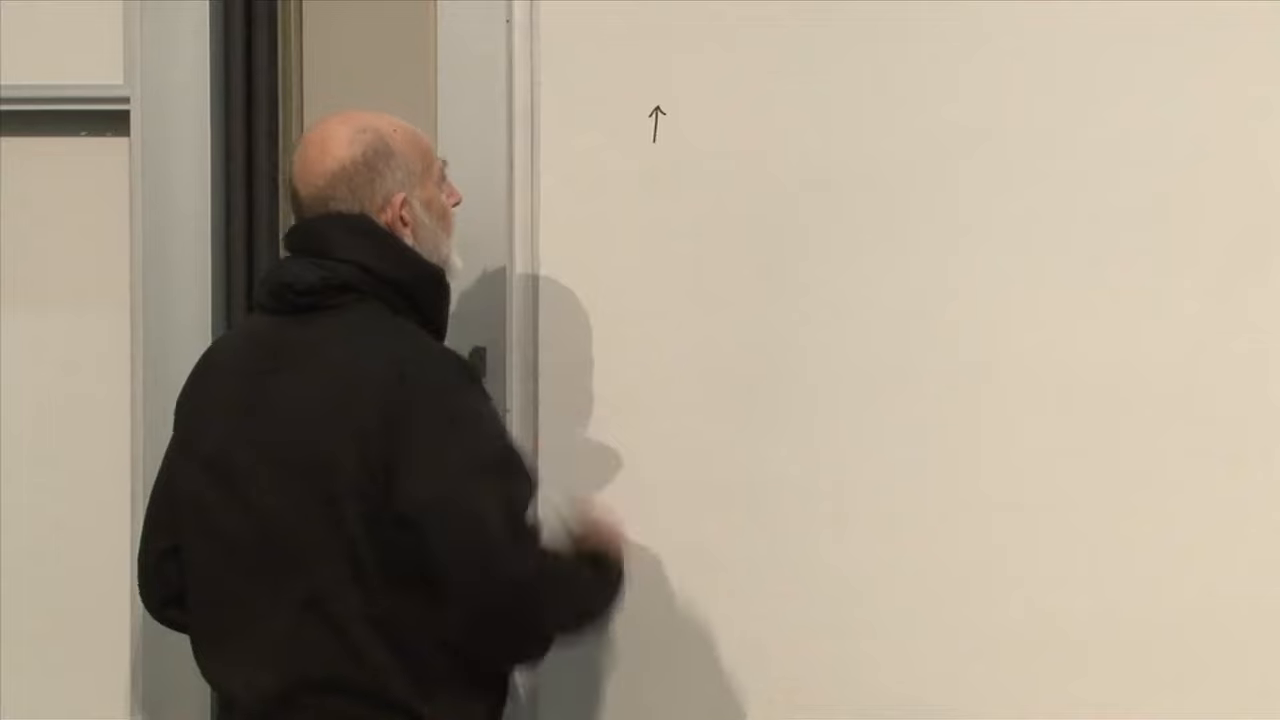
\includegraphics[width=0.64\textwidth]{lecture_02_figure_02.png}
\caption{Ký hiệu tạm thời đầu tiên cho một spin được chuẩn bị dọc theo một trục. Mũi tên gắn nhãn cho một phép chuẩn bị; nó chưa phải là một mô hình cổ điển của trạng thái.}
\lectureframe{00:05:15}
\end{figure}

Chọn các trục sao cho \(z\) hướng lên trên bảng, \(x\) hướng sang phải và \(y\) hướng ra khỏi mặt bảng. Nếu thiết bị được định hướng theo một hướng đơn vị \(\hat m\), thì kết quả của nó là
\begin{equation}
\sigma_{\hat m}=\pm1.
\end{equation}
Cụ thể,
\[
\sigma_z=\pm1,\qquad \sigma_x=\pm1,\qquad \sigma_y=\pm1.
\]
Ở giai đoạn này, từ \emph{thành phần} được hiểu theo nghĩa thao tác: \(\sigma_z\) là giá trị mà thiết bị đã định hướng báo lại khi nó chỉ theo \(z\). Nó chưa phải là thành phần \(z\) của một mũi tên cổ điển ẩn.

\subsection{Tính lặp lại và nhiễu loạn}

Giả sử một phép đo \(z\) cho \(+1\). Nếu không có thao tác xen vào, phép đo \(z\) thứ hai lại cho \(+1\), và các lần lặp tiếp theo cũng vậy. Phép đo thứ nhất đã chuẩn bị một trạng thái trong đó chính câu hỏi ấy có một câu trả lời xác định.

\begin{classroomqa}
\audiencequestion{Nếu một phép đo lượng tử làm nhiễu spin, vì sao một phép lặp lại ngay sau đó lại cho cùng kết quả?}
\lecturerresponse{Sự nhiễu loạn không diễn ra một cách bừa bãi. Việc đo \(\sigma_z\) có thể làm thay đổi điều sẽ xảy ra trong một phép đo theo \(x\) hoặc \(y\) về sau, đồng thời vẫn giữ cho giá trị mới được đo của \(\sigma_z\) có thể tái lập. Một thí nghiệm hữu ích đòi hỏi chính dạng ổn định có giới hạn này.}
\end{classroomqa}

Bây giờ quay thiết bị đi \(180^\circ\). Một spin cho \(+1\) khi thiết bị hướng lên trên sẽ cho \(-1\) khi thiết bị bị lật ngược. Quay thiết bị thẳng đứng trở lại thì kết quả là \(+1\). Vì thế, định hướng là điều quan trọng. Một nhiệt kế sẽ không báo âm của nhiệt độ chỉ vì nó bị lật ngược; bộ phân tích spin hành xử khác vì nó đặt ra một câu hỏi có hướng.

\begin{figure}[htbp]
\centering
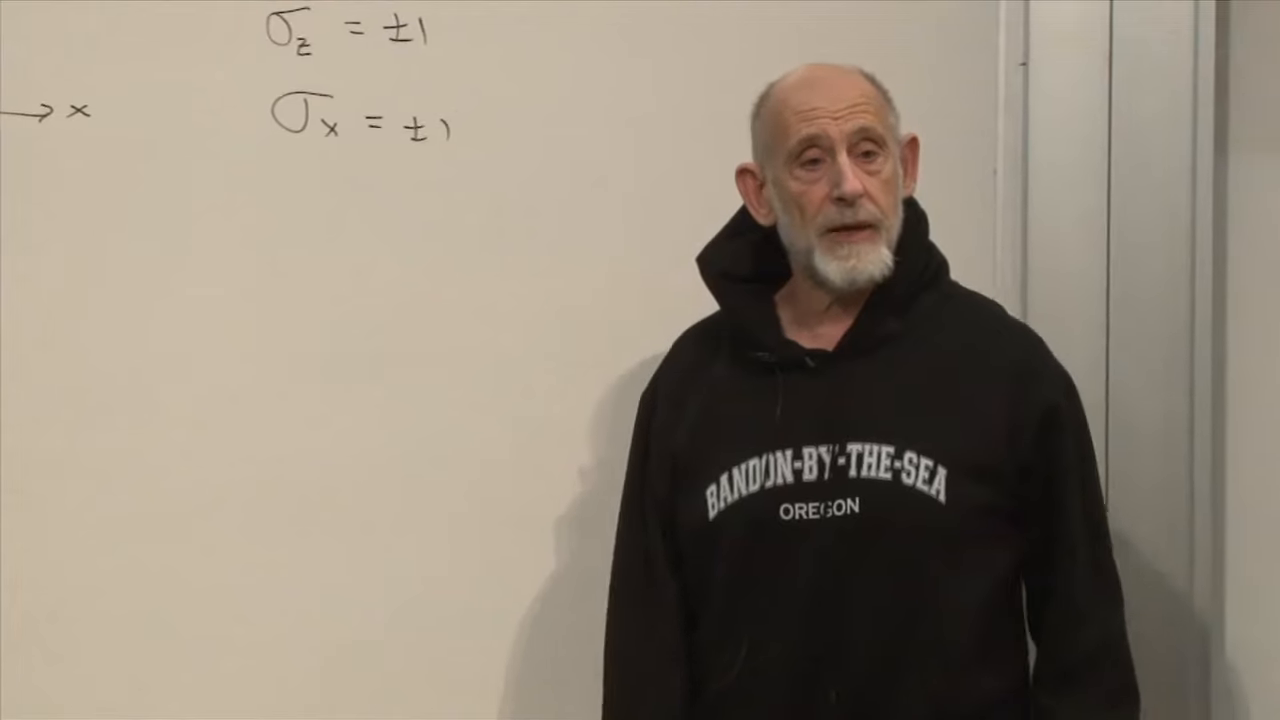
\includegraphics[width=0.72\textwidth]{lecture_02_figure_03.png}
\caption{Bảng ghi lại các nhãn hai giá trị \(\sigma_z=\pm1\) và \(\sigma_x=\pm1\), cùng với dấu hiệu của trục \(x\).}
\lectureframe{00:12:46}
\end{figure}

Sự khác biệt với một vectơ đơn vị cổ điển lộ ra ngay lập tức. Các thành phần cổ điển biến thiên liên tục giữa \(-1\) và \(+1\). Một vectơ đơn vị vuông góc với trục \(x\) có thành phần \(x\) bằng không. Trái lại, một bộ phân tích spin hướng theo \(x\) không bao giờ hiển thị giá trị bằng không. Nó hiển thị \(+1\) hoặc \(-1\), ngay cả khi spin được chuẩn bị dọc theo \(z\).

\section{Kết quả riêng lẻ và các giá trị trung bình dạng vectơ}

Chuẩn bị một spin bằng cách thu được \(\sigma_z=+1\), rồi đo \(\sigma_x\). Một nửa số phép thử được chuẩn bị giống hệt nhau cho \(+1\), và một nửa cho \(-1\). Do đó
\begin{equation}
\langle \sigma_x\rangle=0.
\end{equation}
Sự chuẩn bị ấy cũng cho
\begin{equation}
\langle \sigma_y\rangle=0.
\end{equation}
Ngược lại, một spin được chuẩn bị với \(\sigma_x=+1\) có xác suất bằng nhau cho hai kết quả của một phép đo \(z\) hoặc \(y\) tiếp theo.

Thực ra có hai thí nghiệm khác nhau ẩn trong phát biểu đó. Việc lặp đi lặp lại phép đo \(\sigma_x\) trên chính spin \emph{cùng} đó sau kết quả \(x\) đầu tiên chỉ đơn thuần xác nhận kết quả ấy. Để thu được thống kê năm mươi--năm mươi, cần nhiều spin được chuẩn bị trong cùng trạng thái \(z\), hoặc một spin được đưa trở lại đúng sự chuẩn bị ấy trước mỗi phép đo \(x\).

\begin{classroomqa}
\audiencequestion{Điều gì xảy ra nếu một spin chưa được cố ý chuẩn bị trước khi đi vào thiết bị?}
\lecturerresponse{Kết quả vẫn là \(+1\) hoặc \(-1\), nhưng xác suất của chúng phụ thuộc vào trạng thái mà spin thực sự có. Phép chuẩn bị là quy trình được kiểm soát làm cho các lần thử lặp lại trở nên có thể so sánh được. Nếu có một tác động chưa biết xảy ra giữa hai phép đo, tính lặp lại không còn được bảo đảm; nếu không có gì xảy ra, kết quả của cùng một thành phần là có thể tái lập.}
\end{classroomqa}

\subsection{Hai hướng tùy ý}

Chuẩn bị spin theo một hướng đơn vị \(\hat n\) bằng cách thu được \(+1\) từ một bộ phân tích được định hướng theo \(\hat n\). Sau đó đo theo một hướng đơn vị khác \(\hat m\). Mỗi phép thử vẫn chỉ cho \(\pm1\), nhưng giá trị trung bình trên các phép thử được chuẩn bị giống hệt nhau là
\begin{equation}
\boxed{\langle\sigma_{\hat m}\rangle=\hat n\cdot\hat m
=\cos\theta_{nm}.}
\label{eq:spin-average}
\end{equation}
Trên bảng dùng ký hiệu rút gọn \(\langle\sigma_m\rangle=n\cdot m\):

\begin{figure}[htbp]
\centering
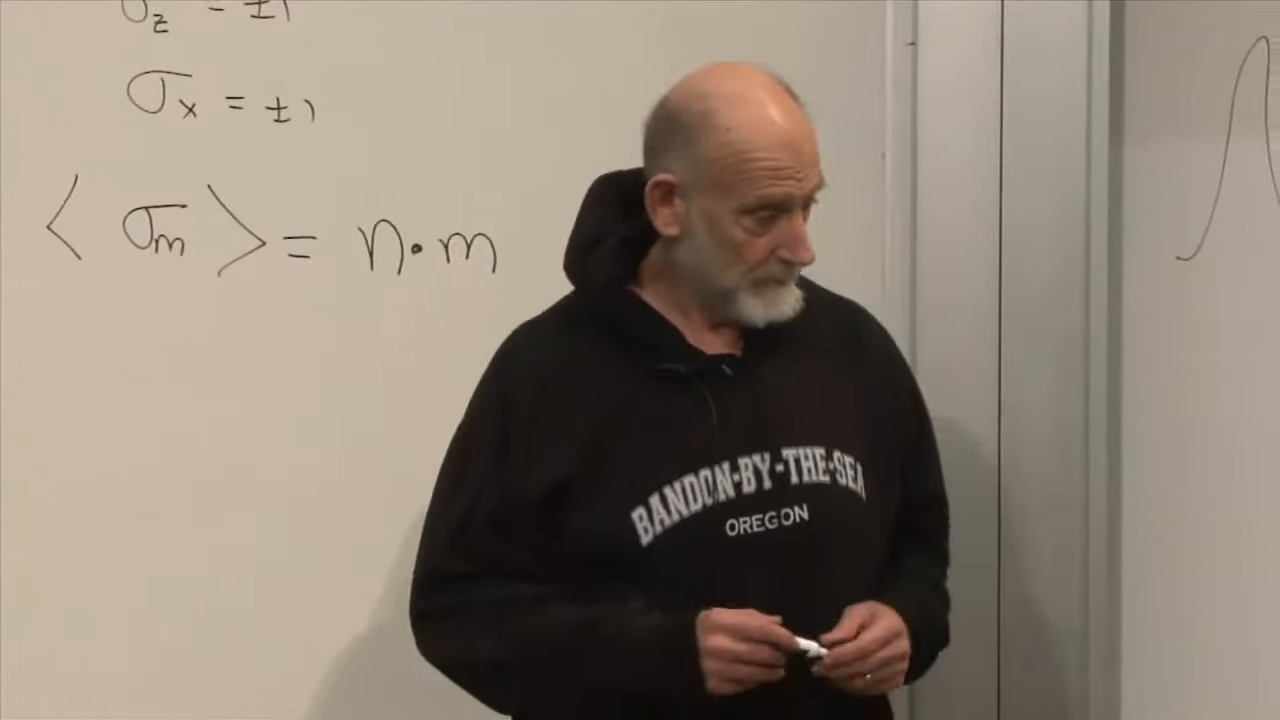
\includegraphics[width=0.74\textwidth]{lecture_02_figure_04.png}
\caption{Định luật dạng vectơ áp dụng cho giá trị trung bình của cả tập hợp, không áp dụng cho một kết quả riêng lẻ \(\pm1\).}
\lectureframe{00:23:22}
\end{figure}

Phương trình~\eqref{eq:spin-average} bao gồm các trường hợp trước đó. Nếu \(\hat m=\hat n\), giá trị trung bình là \(+1\); vì không kết quả nào có thể vượt quá \(+1\), nên mọi phép thử đều cho \(+1\). Nếu \(\hat m=-\hat n\), mọi phép thử đều cho \(-1\). Các trục vuông góc cho giá trị trung bình bằng không và tần suất bằng nhau.

Nếu \(p_+\) và \(p_-\) ký hiệu xác suất của hai kết quả có thể có, thì
\[
p_++p_-=1,\qquad p_+-p_-=\hat n\cdot\hat m.
\]
Do đó,
\begin{equation}
p_\pm=\frac{1\pm\hat n\cdot\hat m}{2}.
\label{eq:direction-probabilities}
\end{equation}
\editorialnote{Bài giảng nêu hai kết quả và giá trị trung bình của chúng. Phương trình~\eqref{eq:direction-probabilities} là hệ quả đại số trực tiếp của hai dữ kiện đó.}

\begin{classroomqa}
\audiencequestion{Đại lượng trong dấu ngoặc góc là một \emph{giá trị kỳ vọng} hay một giá trị trung bình thông thường?}
\lecturerresponse{Đó là trung bình của các kết quả được ghi lại qua nhiều lần lặp. \emph{Giá trị kỳ vọng} là thuật ngữ chuẩn, nhưng ở đây không hàm ý một kiểu lấy trung bình bổ sung nào. Thiết bị tạo ra một danh sách các giá trị \(+1\) và \(-1\); dấu ngoặc biểu thị trung bình cộng của danh sách đó trong giới hạn tập hợp lớn.}
\end{classroomqa}

\begin{classroomqa}
\audiencequestion{Mũi tên \(\hat n\) đã có ý nghĩa hình học ngay từ trước khi biết định luật trung bình hay chưa?}
\lecturerresponse{Ban đầu, nó là một nhãn cho cách thiết bị chuẩn bị được định hướng. Thí nghiệm đảo ngược và sự phụ thuộc của giá trị trung bình vào \(\hat n\cdot\hat m\) mang lại cho nhãn ấy một ý nghĩa hình học thao tác. Thiết bị xác định các thành phần có nghĩa là gì; một kết quả đơn lẻ không bao giờ cung cấp một hình chiếu cổ điển.}
\end{classroomqa}

Đây là sự dung hòa đầu tiên giữa bức tranh định hướng và dữ liệu rời rạc. Spin riêng lẻ không hành xử như một mũi tên cổ điển có các thành phần nhận giá trị liên tục. Tuy nhiên, thống kê của nhiều spin được chuẩn bị giống hệt nhau lại biến đổi đúng hệt như các thành phần của một vectơ ba chiều đơn vị.

\section{Các mệnh đề cổ điển như những tập hợp}

Trước khi xây dựng không gian trạng thái lượng tử, hãy xét logic vận hành như thế nào đối với một hệ cổ điển. Hãy cho các trạng thái khả dĩ tạo thành một tập \(\Omega\). Một mệnh đề \(A\) được biểu diễn bởi tập con các trạng thái mà trên đó \(A\) là đúng.

Đối với một con xúc xắc sáu mặt,
\[
A=\{2,4,6\}
\]
có thể biểu diễn mệnh đề \emph{kết quả là số chẵn}, còn
\[
B=\{4,5,6\}
\]
có thể biểu diễn mệnh đề \emph{kết quả lớn hơn ba}. Các phép toán logic trở thành các phép toán trên tập hợp:
\begin{equation}
\neg A=A^c,\qquad
A\land B=A\cap B,\qquad
A\lor B=A\cup B.
\label{eq:classical-logic}
\end{equation}
Ở đây \(\lor\) là OR bao hàm: \(A\lor B\) là đúng khi \(A\) đúng, \(B\) đúng, hoặc cả hai cùng đúng. Nó không phải là cách dùng loại trừ trong đời thường của \emph{hoặc \(A\) hoặc \(B\), nhưng không phải cả hai}.

\begin{classroomqa}
\audiencequestion{Một phép đo spin chỉ có hai kết quả, nhưng hướng chuẩn bị lại biến thiên liên tục. Tập trạng thái là hữu hạn hay liên tục?}
\lecturerresponse{Tập các hướng chuẩn bị có thể có là liên tục dù mỗi bộ phân tích được chọn chỉ có hai chỉ thị. Chính vì vậy, chỉ đếm các nhãn của detector là không đủ để mô tả không gian trạng thái.}
\end{classroomqa}

Đối với các tập con cổ điển, phép giao và phép hợp không phụ thuộc vào việc mệnh đề nào được nêu trước:
\[
A\cap B=B\cap A,\qquad A\cup B=B\cup A.
\]
Vì thế, một phép kiểm tra thực nghiệm của một mệnh đề ghép cổ điển có thể được lý tưởng hóa mà không cần đưa thứ tự vào logic.

\section{Một phép kiểm tra OR phụ thuộc vào thứ tự}

Xét các mệnh đề lượng tử
\begin{equation}
A:\sigma_z=+1,\qquad B:\sigma_x=+1.
\end{equation}
Mỗi mệnh đề đều có một phép kiểm tra rõ ràng. Hãy định hướng thiết bị theo \(z\) để kiểm tra \(A\), hoặc theo \(x\) để kiểm tra \(B\). Rắc rối xuất hiện khi ta cố xác minh \(A\lor B\) bằng cách kiểm tra một mệnh đề rồi, nếu nó sai, kiểm tra mệnh đề kia.

Hãy tưởng tượng rằng một người chuẩn bị ẩn mặt đã cung cấp một spin hướng lên theo trục \(z\). Nếu \(A\) được kiểm tra trước, kết quả chắc chắn là \(+1\), và phép kiểm tra OR kết thúc với giá trị \emph{đúng}.

Đảo ngược thứ tự. Kiểm tra \(B\) trước cho
\[
P(B)=\frac12,\qquad P(\neg B)=\frac12.
\]
Nếu \(B\) sai, thì phép đo \(x\) dù vậy vẫn đã chuẩn bị một trạng thái \(x\) xác định. Kiểm tra \(A\) trên trạng thái đó cho
\[
P(A\mid \neg B)=\frac12,\qquad
P(\neg A\mid \neg B)=\frac12.
\]
Vì thế, quy trình đảo ngược báo cả hai mệnh đề đều sai với xác suất
\begin{equation}
P(\neg B\ \text{then}\ \neg A)
=\frac12\cdot\frac12=\frac14.
\end{equation}
Một cách sắp xếp luôn chấp nhận phép OR; cách kia bác bỏ nó trong một phần tư số lần thử.

\begin{classroomqa}
\audiencequestion{Sự mâu thuẫn ấy có phải chỉ do ta biết không đầy đủ về trạng thái được bí mật chuẩn bị hay không?}
\lecturerresponse{Không. Sự chuẩn bị ẩn đó chỉ được chọn để làm cho phép so sánh trở nên rành mạch. Phép đo \(x\) đầu tiên về mặt vật lý chuẩn bị một trạng thái \(x\), vì thế phép kiểm tra \(z\) về sau được thực hiện trên một trạng thái đã thay đổi. Việc cho người quan sát thêm thông tin về sự chuẩn bị ban đầu không thể hoàn tác sự can thiệp ấy.}
\end{classroomqa}

\begin{classroomqa}
\audiencequestion{Liệu phép OR có thể được kiểm tra bằng một hệ phân cấp câu hỏi công phu hơn thay vì theo quy tắc tuần tự này không?}
\lecturerresponse{Chắc chắn có thể định nghĩa những quy trình thực nghiệm khác, nhưng khi đó chúng là những phép đo lượng tử khác. Không có một tập con \(A\cup B\) không phụ thuộc vào quy trình mà tính đúng sai của nó đơn giản được bộc lộ bất kể thiết bị nào. Sự phụ thuộc vào thứ tự là lời cảnh báo rằng lôgic tập hợp cổ điển không phải là lôgic tự nhiên của các mệnh đề này.}
\end{classroomqa}

Về sau, các mệnh đề sẽ được biểu diễn bằng các toán tử chiếu. Lời cảnh báo đại số ngắn gọn là
\begin{equation}
P_A P_B\ne P_B P_A.
\end{equation}
Hiện giờ chưa cần thêm gì từ lý thuyết toán tử. Điều quan trọng là các phép kiểm tra không tương thích thì không giao hoán, và các mệnh đề hợp thành của chúng không thể được xử lý như những phép hợp tập hợp thông thường.

\begin{classroomqa}
\audiencequestion{Có thể sắp đặt một phiên bản hai hạt của thí nghiệm này sao cho việc chọn phép kiểm tra tác động ngược về quá khứ không?}
\lecturerresponse{Câu hỏi đó đòi hỏi những công cụ chưa được phát triển ở đây. Không thể rút ra kết luận nào về nhân quả ngược thời gian từ chuỗi một spin, nên vấn đề được để ngỏ thay vì phỏng đoán.}
\end{classroomqa}

\section{Không gian trạng thái tuyến tính}

Một tập hợp chứa các phần tử, nhưng nói chung không có cách tự nhiên nào để cộng hai phần tử và thu được phần tử thứ ba. Một không gian vectơ tuyến tính có nhiều cấu trúc hơn. Nếu \(\ket{A}\) và \(\ket{B}\) là các vectơ và \(\alpha,\beta\in\mathbb C\), thì
\begin{equation}
\alpha\ket{A}+\beta\ket{B}
\end{equation}
là một vectơ khác trong cùng không gian ấy. Các trạng thái lượng tử được biểu diễn trong một không gian tuyến tính phức như vậy.

Với mỗi ket \(\ket{A}\) có một bra đối ngẫu tương ứng \(\bra{A}\). Ghép một bra với một ket cho ra một số phức, gọi là tích trong. Nó tuân theo tính đối xứng liên hợp,
\begin{equation}
\braket{A}{B}=\braket{B}{A}^{*}.
\label{eq:conjugate-symmetry}
\end{equation}

\begin{figure}[htbp]
\centering
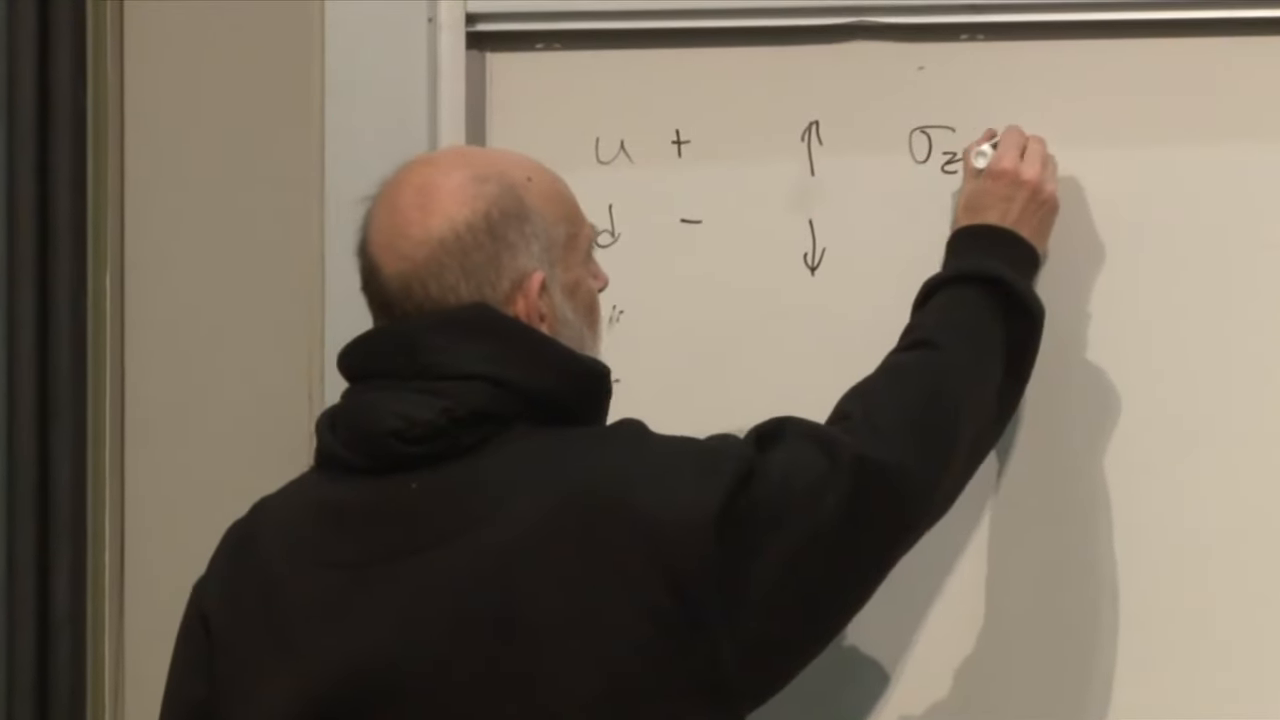
\includegraphics[width=0.78\textwidth]{lecture_02_figure_05.png}
\caption{Bảng tóm tắt các tổ hợp tuyến tính và phép đảo liên hợp của một tích trong.}
\lectureframe{00:46:53}
\end{figure}

Bình phương độ dài của một vectơ là
\begin{equation}
\|\ket{A}\|^2=\braket{A}{A}.
\end{equation}
Phương trình~\eqref{eq:conjugate-symmetry} làm cho số này bằng với liên hợp phức của chính nó, do đó là số thực; các tiên đề của tích trong cũng khiến nó không âm. Hai vectơ trực giao khi
\begin{equation}
\braket{A}{B}=0.
\end{equation}
Số chiều của không gian là số lớn nhất các phương khác không trực giao từng đôi một có thể chọn được.

\begin{classroomqa}
\audiencequestion{Mọi cơ sở có nhất thiết phải gồm các vectơ trực giao từng đôi một không?}
\lecturerresponse{Không. Một cơ sở chỉ cần độc lập tuyến tính và sinh ra không gian. Các cơ sở trực giao đặc biệt thuận tiện vì các hệ số và xác suất dễ rút ra. Trong hai chiều, hai vectơ không song song có thể lập thành một cơ sở ngay cả khi tích trong của chúng không bằng không.}
\end{classroomqa}

\section{Không gian spin hai chiều}

Không gian trạng thái của một spin được giả định bằng hậu đề là một không gian vectơ phức hai chiều,
\begin{equation}
\mathcal H_{\mathrm{spin}}\cong\mathbb C^2.
\end{equation}
Có liên tục vô số vectơ trạng thái khả dĩ, nhưng chỉ cần hai vectơ cơ sở độc lập để biểu diễn bất kỳ vectơ nào trong số đó.

Bắt đầu với các trạng thái được chuẩn bị bởi một thiết bị định hướng theo \(z\):
\begin{align}
\ket{u}&\longleftrightarrow \sigma_z=+1,\\
\ket{d}&\longleftrightarrow \sigma_z=-1.
\end{align}
Các chữ cái \(u,d\), các dấu \(+,-\), và các mũi tên \(\uparrow,\downarrow\) là những nhãn thay thế cho cùng hai cách chuẩn bị đó. Vì một phép đo \(z\) phân biệt chúng một cách chắc chắn, các vectơ trạng thái của chúng trực giao:
\begin{equation}
\braket{u}{d}=0.
\end{equation}
Chọn chúng có độ dài đơn vị,
\[
\braket{u}{u}=\braket{d}{d}=1.
\]

Khi đó, mọi trạng thái spin đều có thể được viết thành
\begin{equation}
\ket{A}=\alpha_u\ket{u}+\alpha_d\ket{d},
\qquad \alpha_u,\alpha_d\in\mathbb C.
\label{eq:general-spin-state}
\end{equation}
Quy tắc xác suất là
\begin{equation}
P(u|A)=|\alpha_u|^2,\qquad
P(d|A)=|\alpha_d|^2.
\label{eq:born-z}
\end{equation}
Vì một trong hai kết quả chắc chắn phải xảy ra,
\begin{equation}
|\alpha_u|^2+|\alpha_d|^2=1.
\label{eq:normalization}
\end{equation}

\begin{figure}[htbp]
\centering
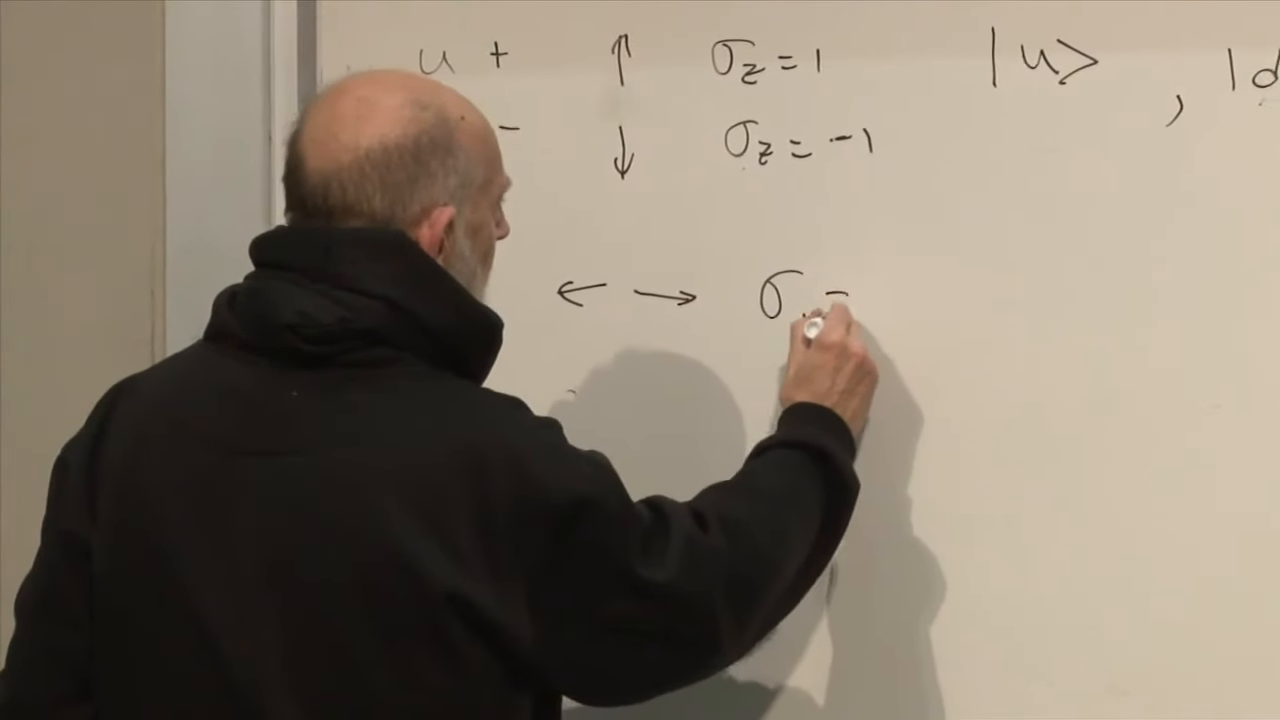
\includegraphics[width=0.78\textwidth]{lecture_02_figure_06.png}
\caption{Khai triển lên--xuống tổng quát, tổng của hai xác suất kết quả, và điều kiện chuẩn đơn vị tương đương.}
\lectureframe{01:03:38}
\end{figure}

Sự tương đương với chuẩn hóa đơn vị suy ra trực tiếp:
\begin{align}
\braket{A}{A}
&=(\alpha_u^*\bra{u}+\alpha_d^*\bra{d})
  (\alpha_u\ket{u}+\alpha_d\ket{d})\\
&=|\alpha_u|^2\braket{u}{u}
 +\alpha_u^*\alpha_d\braket{u}{d}\\
&\quad +\alpha_d^*\alpha_u\braket{d}{u}
 +|\alpha_d|^2\braket{d}{d}\\
&=|\alpha_u|^2+|\alpha_d|^2=1.
\end{align}
Vì vậy, một trạng thái thuần vật lý được biểu diễn bằng một vectơ đã chuẩn hóa.

\begin{classroomqa}
\audiencequestion{Những phát biểu này đang được suy ra, hay là các hậu đề?}
\lecturerresponse{Ở thời điểm này, chúng là những quy tắc đang được khớp với các thí nghiệm. Không gian hai chiều, quy tắc xác suất và cách diễn giải tính trực giao đang được đưa vào theo lối gợi mở. Có thể kiểm tra ngay bây giờ tính nhất quán lẫn nhau của chúng; mối liên hệ có hệ thống giữa trạng thái và đại lượng quan sát sẽ đến tiếp theo.}
\end{classroomqa}

\subsection{Tính trực giao như khả năng phân biệt}

Nội dung vật lý của tính trực giao hữu ích hơn hình ảnh những mũi tên vuông góc:

\begin{quote}
Các trạng thái có thể được phân biệt một cách chắc chắn bằng một phép đo được biểu diễn bằng các vectơ trực giao.
\end{quote}

Lên và xuống thỏa mãn tiêu chuẩn này. Nếu trạng thái là lên, thì thiết bị \(z\) không bao giờ báo xuống, và ngược lại. Một độ chồng lấp khác không cho thấy một trạng thái đôi khi có thể tạo ra kết quả gắn với trạng thái kia.

\section{Cơ sở phải--trái}

Gọi \(\ket{r}\) và \(\ket{l}\) là các trạng thái có spin xác định theo trục \(x\):
\[
\ket{r}\longleftrightarrow\sigma_x=+1,\qquad
\ket{l}\longleftrightarrow\sigma_x=-1.
\]
Vì không gian là hai chiều, mỗi trạng thái phải là một tổ hợp tuyến tính của \(\ket{u}\) và \(\ket{d}\). Một spin được chuẩn bị sang phải cho kết quả lên và xuống với xác suất bằng nhau, nên hai hệ số phải có cùng độ lớn. Chọn quy ước pha đơn giản nhất:
\begin{equation}
\ket{r}=\frac{1}{\sqrt2}\bigl(\ket{u}+\ket{d}\bigr).
\label{eq:right-state}
\end{equation}
Phải và trái được phân biệt một cách chắc chắn bởi thiết bị \(x\), nên trạng thái trái phải trực giao với trạng thái phải. Một lựa chọn thuận tiện là
\begin{equation}
\ket{l}=\frac{1}{\sqrt2}\bigl(\ket{u}-\ket{d}\bigr).
\label{eq:left-state}
\end{equation}
Thật vậy,
\begin{align}
\braket{l}{r}
&=\frac12(\bra{u}-\bra{d})(\ket{u}+\ket{d})\\
&=\frac12(1-1)=0.
\end{align}

\begin{figure}[htbp]
\centering
\includegraphics[width=0.82\textwidth]{lecture_02_figure_07.png}
\caption{Cách xây dựng phải--trái hoàn chỉnh: độ lớn lên--xuống bằng nhau, dấu tương đối đối nhau, và tích trong bằng không.}
\lectureframe{01:12:15}
\end{figure}

Dấu trừ tổng thể của \(\ket{l}\) là quy ước. Thay \(\ket{l}\) bằng \(-\ket{l}\) không làm thay đổi bất kỳ xác suất nào của nó. Cộng và trừ các Phương trình~\eqref{eq:right-state} và~\eqref{eq:left-state} cho phép đổi cơ sở ngược:
\begin{align}
\ket{u}&=\frac{1}{\sqrt2}\bigl(\ket{r}+\ket{l}\bigr),\\
\ket{d}&=\frac{1}{\sqrt2}\bigl(\ket{r}-\ket{l}\bigr).
\end{align}
Tính đối xứng này là quan trọng. Bắt đầu từ cơ sở \(x\), một trạng thái lên hoặc xuống là chồng chập với trọng số bằng nhau của phải và trái, cũng như một trạng thái phải hoặc trái là chồng chập với trọng số bằng nhau của lên và xuống.

\section{Cơ sở vào--ra và pha tương đối}

Định hướng thiết bị dọc theo \(y\), vuông góc với mặt bảng. Viết
\[
\ket{i}\longleftrightarrow\sigma_y=+1,\qquad
\ket{o}\longleftrightarrow\sigma_y=-1,
\]
trong đó nhãn ket \(i\) có nghĩa là \emph{vào}, còn \(i\) đứng riêng khi nhân với một ket vẫn là đơn vị ảo.

Xác suất bằng nhau cho lên và xuống đòi hỏi các hệ số có cùng độ lớn. Tính trực giao giữa vào và ra đòi hỏi một pha tương đối làm cho độ chồng lấp của chúng triệt tiêu. Một lựa chọn đối xứng là
\begin{align}
\ket{i}&=\frac{1}{\sqrt2}\bigl(\ket{u}+i\ket{d}\bigr),\\
\ket{o}&=\frac{1}{\sqrt2}\bigl(\ket{u}-i\ket{d}\bigr).
\label{eq:in-out-states}
\end{align}
Trong cơ sở \((u,d)\), cả sáu trạng thái là
\begin{align}
\ket{u}&=\binom10,
&
\ket{d}&=\binom01,
\\
\ket{r}&=\frac1{\sqrt2}\binom11,
&
\ket{l}&=\frac1{\sqrt2}\binom1{-1},
\\
\ket{i}&=\frac1{\sqrt2}\binom1{i},
&
\ket{o}&=\frac1{\sqrt2}\binom1{-i}.
\end{align}

\begin{figure}[htbp]
\centering
\includegraphics[width=0.82\textwidth]{lecture_02_figure_08.png}
\caption{Sáu vectơ cột trong cơ sở lên--xuống. Cặp ở dưới chỉ khác nhau ở dấu của pha ảo tương đối.}
\lectureframe{01:20:50}
\end{figure}

Phép liên hợp phức trong bra là thiết yếu cho việc kiểm tra tính trực giao:
\begin{align}
\braket{i}{o}
&=\frac12(\bra{u}-i\bra{d})(\ket{u}-i\ket{d})\\
&=\frac12\bigl(1+(-i)(-i)\bigr)=0.
\end{align}

\begin{classroomqa}
\audiencequestion{Việc chọn \(+i\) cho \emph{vào} thay vì \emph{ra} có mã hóa tính tay phải hay tay trái của các trục không gian không?}
\lecturerresponse{Một quy ước đã được đưa vào, và ý nghĩa hình học của nó sẽ rõ ràng hơn khi các ma trận Pauli và các phép quay được phát triển. Hiện tại, cặp này phải trực giao và có quan hệ đối xứng với các cơ sở khác; việc hoán đổi các nhãn hoặc đảo chiều trục \(y\) làm thay đổi quy ước, chứ không làm thay đổi tính nhất quán của cách xây dựng.}
\end{classroomqa}

\subsection{Kiểm tra tính đối xứng trong cơ sở phải--trái}

Dùng
\[
\ket{u}=\frac{\ket{r}+\ket{l}}{\sqrt2},\qquad
\ket{d}=\frac{\ket{r}-\ket{l}}{\sqrt2}
\]
trong trạng thái vào:
\begin{align}
\ket{i}
&=\frac1{\sqrt2}
\left(
\frac{\ket{r}+\ket{l}}{\sqrt2}
+i\frac{\ket{r}-\ket{l}}{\sqrt2}
\right)\\
&=\frac{1+i}{2}\ket{r}
 +\frac{1-i}{2}\ket{l}.
\label{eq:in-in-rl}
\end{align}
Mặc dù không hệ số nào hiển nhiên chứa \(1/\sqrt2\),
\begin{equation}
\left|\frac{1+i}{2}\right|^2
=\left|\frac{1-i}{2}\right|^2
=\frac12.
\end{equation}

\begin{figure}[htbp]
\centering
\includegraphics[width=0.82\textwidth]{lecture_02_figure_09.png}
\caption{Việc đổi cơ sở trực tiếp cho trạng thái vào và phép kiểm tra rằng mỗi xác suất phải--trái đều bằng \(1/2\).}
\lectureframe{01:29:10}
\end{figure}

Vì vậy, mỗi trạng thái trong một trong ba cơ sở đều cho các xác suất bằng nhau khi được đo trong một trong hai cơ sở còn lại. Các cơ sở \(z\), \(x\) và \(y\) là không thiên lệch lẫn nhau.

\section{Vì sao có ba cặp cơ sở đặc biệt}

\begin{classroomqa}
\audiencequestion{Có thể có một cặp trạng thái thứ tư, liên hệ đối xứng với ba cặp này giống như chúng đối xứng với nhau hay không?}
\lecturerresponse{Không, đối với một hệ hai trạng thái đơn lẻ thì không thể. Một khi ba cặp không thiên lệch lẫn nhau đã được cố định, sẽ không có cặp thứ tư nào có cùng quan hệ độ chồng lấp bằng nhau. Việc có ba nhãn không gian như vậy gắn với ba chiều của không gian thông thường, mặc dù chính không gian trạng thái phức chỉ có hai chiều.}
\end{classroomqa}

Mối liên hệ này có thể thấy được bằng cách đếm các tham số vật lý. Một vectơ cột tổng quát
\[
\binom{\alpha_u}{\alpha_d}
\]
chứa hai số phức, do đó là bốn số thực. Chuẩn hóa loại bỏ một tham số:
\[
|\alpha_u|^2+|\alpha_d|^2=1.
\]
Nhân cả hai thành phần với cùng một pha không làm thay đổi xác suất đo nào:
\begin{equation}
\ket{A}\sim e^{i\chi}\ket{A}.
\label{eq:global-phase}
\end{equation}
Điều đó loại bỏ thêm một tham số thực nữa. Vì vậy, còn lại
\begin{equation}
4-1-1=2
\end{equation}
tham số thực vật lý, đúng bằng số góc cần để xác định một phương trong không gian ba chiều.

Một đại diện thuận tiện làm cho mối liên hệ ấy trở nên tường minh:
\begin{equation}
\ket{\psi(\theta,\phi)}
=\cos\frac{\theta}{2}\,\ket{u}
+e^{i\phi}\sin\frac{\theta}{2}\,\ket{d}.
\label{eq:bloch-parameterization}
\end{equation}
\editorialnote{Phương trình~\eqref{eq:bloch-parameterization} là đại diện chuẩn hóa tiêu chuẩn của họ hai tham số được bài giảng xác định. Dạng góc nửa tường minh được đưa vào để làm cho việc đếm tham số trở nên cụ thể; cách diễn giải động lực học và quay của nó thuộc về các bài giảng sau.}

\begin{classroomqa}
\audiencequestion{Toán học chính xác của việc bỏ qua pha tổng thể là gì?}
\lecturerresponse{Mọi vectơ đã chuẩn hóa trên vòng tròn \(\{e^{i\chi}\ket{\psi}\}\) đều biểu diễn cùng một trạng thái vật lý. Người ta đồng nhất các vectơ đó là tương đương, cũng như những điểm liên hệ với nhau bởi một tính dư thừa đã được tuyên bố thì được xem là một điểm vật lý duy nhất. Pha tương đối giữa các thành phần vẫn đo được; chỉ pha nhân lên toàn bộ vectơ mới bị loại bỏ.}
\end{classroomqa}

\begin{classroomqa}
\audiencequestion{Các vectơ chưa chuẩn hóa hoặc các vectơ có thành phần âm vẫn có thể xuất hiện trong một phép tính không?}
\lecturerresponse{Có. Đại số tuyến tính cho phép điều đó, và một vectơ trung gian chưa nhất thiết phải biểu diễn một trạng thái vật lý đã được chuẩn bị. Một vectơ khác không có thể được chuẩn hóa ở bước cuối. Các thành phần âm và phức là biên độ, không phải xác suất âm; xác suất nảy sinh từ bình phương độ lớn sau khi trạng thái đã được chuẩn hóa.}
\end{classroomqa}

\begin{classroomqa}
\audiencequestion{Bức tranh này sẽ ra sao trong các không gian nhiều chiều hơn, hoặc đối với các spinor phức tạp hơn?}
\lecturerresponse{Những nguyên lý tuyến tính ấy vẫn tiếp tục đúng, nhưng mối liên hệ giữa số chiều của không gian trạng thái, các phép quay trong không gian và spin quan sát được trở nên phong phú hơn. Sự mở rộng đó nằm ngoài cách xây dựng hai trạng thái hiện tại.}
\end{classroomqa}

\section{Tính trực giao không phải là sự vuông góc trong không gian}

Từ \emph{trực giao} giờ đây mang một ý nghĩa trừu tượng, có tính thao tác. Không được nhầm nó với góc giữa hai mũi tên vẽ trong không gian thông thường. Các hướng không gian lên và xuống là đối nhau, nhưng các vectơ trạng thái \(\ket{u}\) và \(\ket{d}\) lại trực giao. Các hướng không gian lên và phải là vuông góc, nhưng
\begin{equation}
\braket{u}{r}=\frac1{\sqrt2}\ne0.
\end{equation}

\begin{classroomqa}
\audiencequestion{Làm sao các hướng không gian đối nhau lại có thể trực giao, trong khi các hướng không gian vuông góc thì không?}
\lecturerresponse{Độ chồng lấp trong không gian trạng thái đo khả năng phân biệt bằng thí nghiệm, chứ không phải góc Euclid giữa các nhãn. Lên và xuống có thể được phân biệt chắc chắn bằng một phép đo \(z\), nên độ chồng lấp của chúng triệt tiêu. Lên và phải thì không thể: một spin được chuẩn bị sang phải đôi khi cho kết quả lên. Vì vậy, các vectơ trạng thái của chúng có chồng lấp.}
\end{classroomqa}

Cùng ý tưởng ấy có một phép tương tự xác suất cổ điển. Hai phân bố xác suất có miền hỗ trợ rời nhau thì phân biệt được hoàn hảo: một kết quả quan sát được sẽ xác định phân bố nào đã được dùng. Các phân bố có miền hỗ trợ chồng lấn không thể được phân biệt mà không mắc sai số chỉ từ một mẫu. Tính trực giao lượng tử đóng vai trò của sự không chồng lấn, còn một tích trong khác không báo hiệu rằng một số kết quả tương thích với cả hai cách chuẩn bị.

\begin{classroomqa}
\audiencequestion{Có nên hình dung không gian trạng thái hai chiều như là mặt phẳng vật lý chứa các mũi tên lên và sang phải không?}
\lecturerresponse{Không. Các nhãn \(x,y,z\) chỉ các định hướng của thiết bị trong không gian thông thường. Các ket thuộc về một không gian vectơ phức với tích trong riêng của nó. Số tham số cho thấy mối liên hệ giữa hai cấu trúc này, nhưng nếu đồng nhất hình ảnh của chúng từng điểm một thì sẽ nhầm lẫn tính vuông góc trong không gian với tính trực giao trong không gian trạng thái.}
\end{classroomqa}

\section{Trạng thái, phép đo, và những gì còn phải làm}

Cho đến nay, việc xây dựng đã được tiến hành bằng cách khớp các vectơ với các dữ kiện thao tác. Ba định hướng của thiết bị gắn nhãn cho ba cặp trạng thái đã chuẩn hóa, và các độ chồng lấp tái tạo các xác suất quan sát được. Một trình bày chặt chẽ vẫn còn phải nói rõ một đại lượng quan sát như \(\sigma_z\) tác dụng lên một trạng thái như thế nào và vì sao các kết quả khả dĩ của nó lại là các trị riêng của nó. Đó là bước tiếp theo.

Câu đố logic trước đó nay có thể được phát biểu sắc nét hơn. Các mệnh đề tương ứng với các không gian con hoặc các toán tử chiếu của chúng, và các toán tử chiếu bất tương hợp thì không giao hoán. Phép thử HOẶC nhạy với thứ tự không phải là một nghịch lý ngôn từ; đó là một sự xuất hiện sớm của cấu trúc không giao hoán này.

\begin{classroomqa}
\audiencequestion{Nếu trạng thái không phải là một mũi tên thông thường, thì vì sao ba nhãn \(x,y,z\) và giá trị trung bình \(\langle\sigma_{\hat m}\rangle\) lại có vẻ cổ điển đến vậy?}
\lecturerresponse{Vectơ cổ điển xuất hiện trong các trung bình theo tập hợp. Một spin đơn lẻ cho một câu trả lời rời rạc, còn nhiều spin được chuẩn bị giống hệt nhau cho ra các giá trị trung bình biến đổi như các thành phần của một hướng. Hành vi cổ điển vĩ mô xuất hiện khi các tập hợp lớn làm cho các giá trị trung bình ấy ổn định; không nên hiểu ngược lại rằng trong mỗi spin riêng lẻ đều có một giá trị liên tục ẩn.}
\end{classroomqa}

\begin{classroomqa}
\audiencequestion{Sự dư thừa của pha chung có phải là một ví dụ của bất biến chuẩn không?}
\lecturerresponse{Đó là một bất biến đơn giản đối với một pha chung, và nó báo trước những ý tưởng chuẩn rộng hơn. Triển khai mối liên hệ đó ở đây sẽ vượt quá khuôn khổ của cách xây dựng hiện tại, nên chỉ giữ lại mệnh đề có ý nghĩa vật lý: pha chung là không quan sát được, pha tương đối thì không phải vậy.}
\end{classroomqa}

Cuối cùng, không nên hình dung một phép đo chỉ đơn thuần là bộc lộ một giá trị mà spin đã mang sẵn theo nghĩa cổ điển ngay từ đầu. Nó chuẩn bị trạng thái gắn với kết quả được ghi nhận. Vì thế, việc lặp lại ngay lập tức cùng phép đo sẽ cho kết quả nhất quán, trong khi một tập hợp mới gồm các spin được chuẩn bị giống hệt nhau lại biểu lộ phân bố xác suất do các biên độ liên quan quyết định. Mô tả toán học của sự chuẩn bị và việc đọc kết quả đó sẽ trở nên chính xác một khi các đại lượng quan sát được đưa vào như các toán tử.
